\documentclass[11pt,a4paper]{article}
\usepackage[a4paper,top=2cm,bottom=2cm,left=2.1cm,right=2.1cm]{geometry}
\usepackage{fontspec}
\usepackage{polyglossia}
\setdefaultlanguage{spanish}
\setmainfont{TeX Gyre Pagella}
\setsansfont{TeX Gyre Heros}
\usepackage{unicode-math}
\setmathfont{DejaVu Math TeX Gyre}
\usepackage{graphicx}
\usepackage{booktabs}
\usepackage{caption}
\usepackage{xcolor}
\usepackage{titlesec}
\usepackage{enumitem}
\usepackage[hidelinks]{hyperref}
\captionsetup{font=small,labelfont=bf,labelsep=period}
\titleformat{\section}{\sffamily\bfseries\large}{\thesection.}{0.5em}{}
\titleformat{\subsection}{\sffamily\bfseries\normalsize}{\thesubsection.}{0.5em}{}
\titlespacing*{\section}{0pt}{1.0ex plus .4ex}{0.5ex}
\titlespacing*{\subsection}{0pt}{0.8ex plus .3ex}{0.3ex}
\setlength{\parskip}{0.35em}
\setlength{\parindent}{0pt}
\setlist{nosep,leftmargin=1.2em}
\linespread{1.03}

\begin{document}

{\sffamily\bfseries\Large Segmentación de lesiones hipermetabólicas en FDG-PET/CT de cuerpo entero: fusión temprana frente a fusión intermedia con atención cruzada\par}
\vspace{0.4em}
{\small BME423 Procesamiento de imágenes médicas, segundo semestre 2026. Entrega parcial del mini-proyecto.\\
Sebastián Inostroza, Tecnólogo Médico, Doctorado en Ciencias e Ingeniería para la Salud, Universidad de Valparaíso. Modalidad individual.\\
Repositorio: rama \texttt{main}, etiqueta \texttt{resultados-validacion-4-brazos}.\par}
\vspace{0.6em}

\section{Estado del avance}

Esta entrega reporta lo que hice entre el 3 y el 12 de septiembre de 2026: el pipeline completo, la referencia clásica, los tres modelos comprometidos en la definición de tema (A, B y C) y un cuarto brazo (E), cada uno entrenado con tres semillas y evaluado en validación. El conjunto de prueba sigue cerrado.

El resultado central es negativo para la hipótesis. Las cuatro formas de combinar PET y CT empatan: ninguna diferencia entre arquitecturas resiste una comparación pareada por estudio. Todas, en cambio, superan al umbral clásico por un factor de 57 en volumen de falso positivo. La atención cruzada del modelo C quedó inerte y pude medir por qué. Encontré también que el criterio para elegir el checkpoint mete más variación en el falso positivo que la semilla.

\section{Problema, objetivo e hipótesis}

El FDG marca consumo de glucosa, no tumor. Encéfalo, miocardio, riñones, vía urinaria e intestino captan de forma fisiológica, y la inflamación lo hace de forma patológica pero no maligna. Un umbral de SUV no distingue esos tejidos de una lesión, y cada mililitro de falso positivo infla el volumen tumoral metabólico (MTV) que se usa en el seguimiento.

El objetivo es comparar tres estrategias de fusión PET/CT en una U-Net 3D con el mismo presupuesto de datos e iteraciones, y medir su efecto sobre el falso positivo en órganos de captación fisiológica. La hipótesis, sin cambios desde la definición: condicionar las activaciones del PET a la evidencia anatómica del CT mediante atención cruzada reduce el volumen de falso positivo (FPV) respecto de la fusión temprana, sin aumentar el volumen de falso negativo (FNV).

\section{Qué implementé}

\subsection{Datos y preprocesamiento}

Uso la colección FDG-PET-CT-Lesions de TCIA (autoPET, versión anonimizada, CC BY 4.0) [1]. El subconjunto de trabajo tiene 251 estudios de 251 pacientes distintos, sorteados con semilla 423: 201 positivos (67 de pulmón, 67 de linfoma, 67 de melanoma) y 50 controles. La partición es por paciente, 176 de entrenamiento, 26 de validación y 49 de prueba. El manifiesto no cambió desde su creación (md5 registrado en \texttt{docs/PROTOCOLO\_CONGELADO.md}).

La conversión DICOM a NIfTI calcula el SUV normalizado por peso y corrige la orientación del DICOM SEG para que coincida con la del PET. Remuestreo a 3 mm isotrópicos, ventana del CT de $-200$ a 300 HU llevada a $[0,1]$, SUV dividido por 30 con tope, máscara corporal y recorte a la caja del cuerpo. Todas las constantes son fijas, de modo que el preprocesamiento no aprende nada de validación ni de prueba.

Al revisar los datos encontré lesiones anotadas dentro de la caja que la anonimización borra, donde el SUV vale cero: 1\,651 de los 44\,414 mL anotados en los 251 estudios (3,7\,\%). Ningún método puede detectarlas porque no queda señal. Las excluyo de la predicción y de la verdad en la evaluación, con la misma regla para todos los brazos, y reporto ambas métricas, corregida y cruda.

\subsection{Referencia clásica y modelos}

La referencia clásica aplica umbral SUV $\geq 2{,}5$, apertura morfológica de radio 1, componentes de al menos 0,5 mL y exclusión anatómica de órganos fisiológicos. Los parámetros se fijaron en el diseño, sin mirar validación.

\begin{itemize}
\item \textbf{A}, fusión temprana: SUV y CT como dos canales de una U-Net 3D de MONAI [9] (canales 32, 64, 128, 256, 320; 12,9 M parámetros).
\item \textbf{B}, fusión intermedia: un codificador por modalidad y concatenación en el cuello de botella (24,0 M). Es el control de capacidad de C.
\item \textbf{C}, B más un bloque de atención cruzada en el cuello de botella, con el PET como consulta y el CT como clave y valor, mezclado por un factor aprendido $\gamma$ (24,4 M). Con parches de $96^3$ el cuello tiene 216 posiciones.
\item \textbf{E}, brazo agregado: A con un tercer canal, el SUV dividido por la captación hepática del propio paciente. Lo sumé el 10 de septiembre porque el atlas de captación normal que construí con 35 controles reproduce los valores publicados (hígado, mediana 2,19) y la clínica ya usa el hígado como referencia interna (criterio de Deauville). Si la red recibe esa referencia, debería separar mejor captación normal de lesión.
\end{itemize}

\subsection{Entrenamiento y protocolo}

Las doce corridas comparten todo salvo la arquitectura y la semilla (423, 2, 3): 25\,000 iteraciones, lote de 2 parches de $96^3$, 70\,\% de parches centrados en lesión, volteos laterales y anteroposteriores, AdamW con tasa $3\cdot10^{-4}$ y programa polinomial, pérdida Dice más entropía cruzada. Entreno en un Mac con Apple Silicon (acelerador \texttt{mps}, 24 GB, fp32), entre 5 y 6,5 horas por corrida. El 6 de septiembre congelé el protocolo y audité fugas de información: ningún paciente en dos particiones, ninguna estadística global, prueba sin abrir.

Las métricas por estudio son Dice en positivos (Dice$^+$), FPV y FNV, con componentes 26-conexas. Comparo brazos con bootstrap pareado por estudio (IC 95\,\%) y prueba de Wilcoxon, usando la media de las tres semillas por estudio. El falso positivo se reparte por órgano con mapas de TotalSegmentator calculados sobre el CT, que se usan solo para evaluar.

\section{Resultados en validación}

\begin{table}[h]
\centering\small
\caption{Validación, 26 estudios (20 positivos evaluables). Media $\pm$ desviación entre tres semillas. \texttt{mejor.pt} es el checkpoint del protocolo; \texttt{ultimo.pt}, la iteración 25\,000.}
\begin{tabular}{lcccccc}
\toprule
 & \multicolumn{3}{c}{\texttt{mejor.pt}} & \multicolumn{3}{c}{\texttt{ultimo.pt}} \\
\cmidrule(lr){2-4}\cmidrule(lr){5-7}
Brazo & Dice$^+$ & FPV (mL) & FNV (mL) & Dice$^+$ & FPV (mL) & FNV (mL) \\
\midrule
A & 0,621 $\pm$ 0,016 & 20,9 $\pm$ 2,5 & 6,0 & 0,615 $\pm$ 0,020 & 21,7 $\pm$ 0,5 & 5,9 \\
B & 0,612 $\pm$ 0,014 & 22,8 $\pm$ 3,1 & 5,4 & 0,607 $\pm$ 0,002 & 22,1 $\pm$ 2,8 & 4,4 \\
C & 0,612 $\pm$ 0,008 & 23,2 $\pm$ 6,7 & 5,9 & 0,610 $\pm$ 0,007 & 21,5 $\pm$ 1,8 & 4,5 \\
E & 0,640 $\pm$ 0,022 & 22,0 $\pm$ 9,8 & 7,3 & 0,638 $\pm$ 0,006 & 23,6 $\pm$ 2,8 & 5,7 \\
Clásica & 0,180 & 1\,191,9 & 5,6 & & & \\
\bottomrule
\end{tabular}
\end{table}

\textbf{Las fusiones empatan.} Frente a A, la diferencia pareada de Dice$^+$ es $-0{,}009$ para B (IC $-0{,}055$ a $+0{,}024$; $p=0{,}52$), $-0{,}009$ para C ($-0{,}061$ a $+0{,}030$; $p=0{,}87$) y $+0{,}018$ para E ($-0{,}020$ a $+0{,}062$; $p=0{,}93$). Todos los intervalos cruzan el cero. Con 176 estudios de entrenamiento y este presupuesto, la forma de fusionar no cambia el resultado. Por diagnóstico, el Dice de A es 0,74 en pulmón, 0,70 en linfoma y 0,40 en melanoma, y el orden se repite en los demás brazos.

\textbf{Las redes resuelven el falso positivo anatómico.} El umbral clásico deja 1\,192 mL de falso positivo por estudio, y el 74\,\% (879 mL) cae en órganos de captación fisiológica: hígado 349, corazón 142, vejiga 132, riñones 112, intestino 103. En las redes ese error baja a 21 a 23 mL por estudio (Figura~\ref{fig:fp}). Lo que les queda está sobre todo en tejido blando no clasificado e intestino, y no hay diferencia entre A, B y C en ningún órgano.

\begin{figure}[h]
\centering
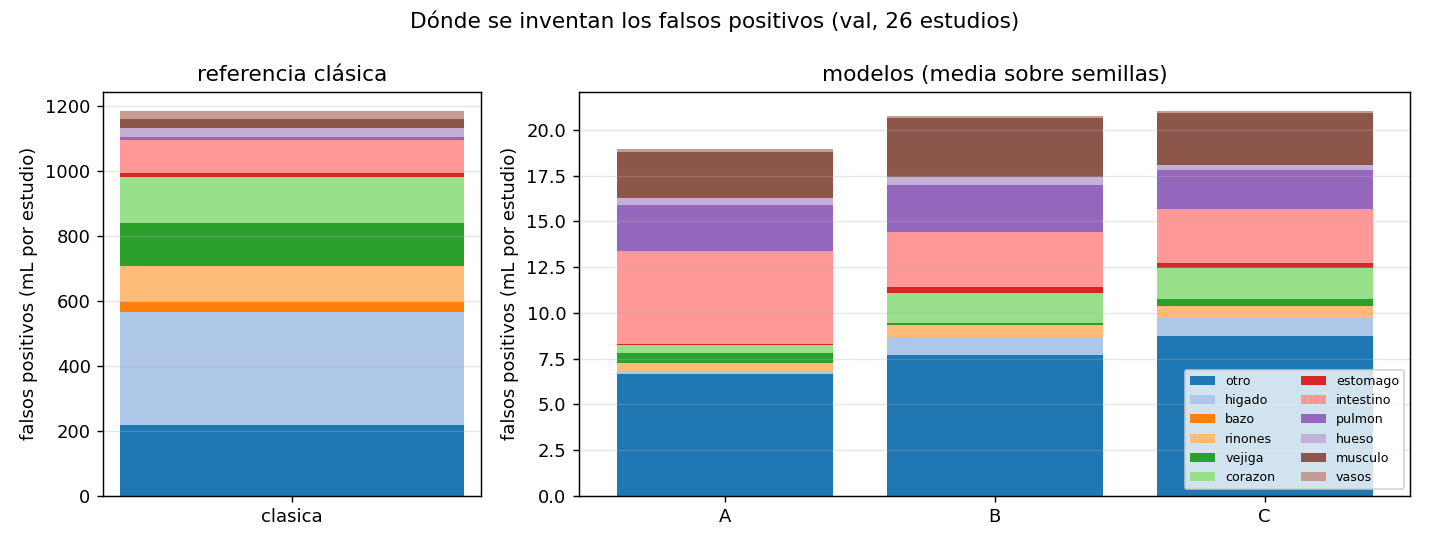
\includegraphics[width=0.86\linewidth]{figuras/fp_por_organo_val.png}
\caption{Falso positivo por órgano en validación (mL por estudio). La barra del método clásico (1\,192 mL) está dominada por órganos de captación fisiológica; las tres redes quedan cerca de 21 mL.}
\label{fig:fp}
\end{figure}

\textbf{La detección depende del tamaño de la lesión, no del diagnóstico.} De las 256 lesiones de validación, las redes detectan prácticamente todas las de más de 10 mL y solo una de cada cinco bajo 1 mL (Tabla~\ref{tab:tam}). Eso explica el Dice bajo en melanoma, cuyas lesiones miden entre 3 y 9 mL, en plena zona de transición. Medida como volumen a corregir, la predicción de A ahorra el 57\,\% del trabajo frente a delinear desde cero (64,6 contra 151,7 mL por estudio). Un ensamble por voto de las tres semillas sube A a Dice$^+$ 0,662 (IC 0,559 a 0,757) y baja el FPV a 17,1 mL sin entrenar nada nuevo. La MTV automática subestima en promedio 30,2 mL, con límites de concordancia de $-244{,}5$ a $+184{,}1$ mL: todavía no sirve para seguir respuesta en pacientes de carga alta.

\begin{table}[h]
\centering\small
\caption{Fracción de lesiones detectadas según tamaño (validación, media de tres semillas).}
\label{tab:tam}
\begin{tabular}{lcccccc}
\toprule
Tamaño & $<1$ mL & 1 a 3 mL & 3 a 10 mL & 10 a 30 mL & 30 a 100 mL & $\geq 100$ mL \\
Lesiones & 100 & 75 & 43 & 24 & 8 & 6 \\
\midrule
A & 0,22 & 0,58 & 0,81 & 1,00 & 1,00 & 1,00 \\
B & 0,23 & 0,63 & 0,83 & 1,00 & 1,00 & 1,00 \\
C & 0,21 & 0,56 & 0,86 & 0,99 & 1,00 & 1,00 \\
\bottomrule
\end{tabular}
\end{table}

\section{Lo que no funcionó y por qué}

\textbf{La atención de C está muerta.} Al forzar $\gamma=0$ en el modelo entrenado, la predicción no cambia en un solo vóxel: diferencia de Dice 0,000 en los 26 estudios y en las tres semillas. Con $\gamma$ inicial en 0 la red lo dejó en 0,0125; con $\gamma$ inicial en 1 terminó entre 0,985 y 1,005, y aun así la ablación dio cero. El mecanismo es que la atención aprendió pesos casi uniformes sobre las 216 posiciones, de modo que su salida es un vector igual en todo el cuello de botella, y la normalización de instancia que sigue resta la media espacial y lo borra. La rama de atención queda conectada pero sin efecto. Para que la anatomía module al PET por esta vía haría falta mover la atención a niveles de mayor resolución o cambiar la normalización.

\textbf{El canal de E está vivo, pero no paga.} Si reemplazo la referencia hepática del paciente por una constante poblacional, cambian 23 de 26 predicciones. El efecto neto es de 1,4 mL de FPV, menor que la variación entre semillas. Su ventaja aparente en Dice venía del checkpoint elegido.

\textbf{El checkpoint pesa más que la semilla.} \texttt{mejor.pt} se elige con el máximo Dice de una validación rápida de 12 estudios. Al usar en cambio el checkpoint final, la desviación del FPV entre semillas baja 5,1 veces en A, 3,8 en C y 3,4 en E, mientras el Dice medio cambia apenas 0,005 y el orden entre modelos se mantiene. Elegir el máximo de una curva ruidosa optimiza una métrica y deja las otras al azar. No estaba en el plan y es el hallazgo mejor sostenido de esta fase, porque está medido en doce corridas independientes.

\section{Ajustes respecto de la definición de tema}

Declaro las diferencias entre lo comprometido y lo hecho, para que la entrega final sea consistente con esta.

\begin{itemize}
\item \textbf{Hausdorff 95.} Comprometido y aún no implementado. Lo agrego para la final, calculado en positivos y sobre la misma máscara corregida.
\item \textbf{Script oficial de autoPET.} Las métricas son una implementación propia con las mismas definiciones (Dice, FPV y FNV por componentes 26-conexas), con pruebas unitarias. En la final la contrasto contra el script oficial sobre los mismos estudios.
\item \textbf{Error en MTV y SUVmax.} La concordancia de MTV está hecha; el error de SUVmax por paciente queda para la final.
\item \textbf{Exclusión de la zona anonimizada}, explicada en la sección 3.1. Con ella el trabajo no dice nada sobre cabeza y cuello ni sobre la captación cerebral.
\item \textbf{Brazo E}, agregado con la justificación de la sección 3.2. No reemplaza a ninguno de los comprometidos.
\item \textbf{Duración.} Planifiqué nueve horas por corrida; en la práctica fueron entre 5 y 6,5, lo que permitió doce corridas en vez de nueve.
\end{itemize}

\section{Plan hacia la entrega final}

El empate se explica bien por falta de datos: con 176 estudios de entrenamiento ninguna arquitectura tiene de dónde aprender la diferencia entre captación fisiológica y lesión. Por eso la siguiente etapa, en la rama \texttt{extendido} del repositorio, entrena con todos los estudios disponibles fuera de la prueba (825), cuatro veces más iteraciones (100\,000) y un ensamble de cinco pliegues con evaluación fuera de pliegue. Los primeros números en validación son preliminares y no forman parte de los resultados de esta entrega: a 100\,000 iteraciones B llega a Dice$^+$ 0,705 frente a 0,694 de A, y el ensamble con volteos en inferencia a 0,754 con FPV de 9,2 mL.

La prueba de 49 estudios se abre una sola vez, con todos los brazos de las dos etapas a la vez. Antes de abrirla dejé escritas y versionadas en git las hipótesis, el sistema final, los umbrales y los criterios de éxito, y el script de evaluación se niega a correr si esos archivos tienen cambios sin registrar. Para la final quedan también el Hausdorff 95, el error de SUVmax, la contrastación con el script oficial, el análisis cualitativo de casos y el informe en LaTeX con su presentación.

\section{Trabajo realizado}

La rama \texttt{main} tiene 64 commits en diez días de trabajo, del 3 al 12 de septiembre, más una bitácora fechada, un glosario y los cuadernos ejecutados. Los hitos:

{\small
\begin{tabular}{@{}p{1.6cm}p{14.6cm}@{}}
\toprule
3 sep & Estructura del repositorio, cálculo de SUV, conversión DICOM a NIfTI, pruebas con fantoma sintético, corrección de orientación del DICOM SEG, geometría de PET y CT. \\
4 sep & Los 251 estudios convertidos y preprocesados; dataset de parches, modelo A y bucle de entrenamiento; medición de velocidad en el Mac. \\
5 sep & A entrenado (FPV de 1\,192 a 18 mL); modelos B y C; hallazgo de lesiones en la zona anonimizada y regla de exclusión. \\
6 sep & Protocolo congelado y auditoría de fugas; B cerrado con tres semillas; ablación de la atención de C. \\
7 a 8 sep & C reentrenado con $\gamma$ inicial 1, segunda ablación nula, mecanismo identificado; falso positivo por órgano. \\
9 a 10 sep & Detección por tamaño, carga de corrección, ensamble, MTV; costo del criterio de checkpoint; atlas de captación normal; modelo E. \\
11 a 12 sep & Desfase PET-CT en el diafragma (200 estudios), evaluación y ablación de E, corte de resultados de los cuatro brazos. \\
\bottomrule
\end{tabular}}

\section*{Referencias}\sloppy
{\small
\begin{enumerate}[label={[\arabic*]},leftmargin=2em]
\item Gatidis S, et al. A whole-body FDG-PET/CT dataset with manually annotated tumor lesions. Sci Data. 2022;9:601.
\item Gatidis S, et al. Results from the autoPET challenge on fully automated lesion segmentation in oncologic PET/CT imaging. Nat Mach Intell. 2024;6:1396-1405.
\item Isensee F, Maier-Hein KH. Look Ma, no code: fine tuning nnU-Net for the autoPET II challenge by only adjusting its JSON plans. arXiv:2309.13747; 2023.
\item Alloula A, McGowan DR, Papież BW. autoPET challenge 2023: nnU-Net-based whole-body 3D PET-CT tumour segmentation. arXiv:2309.13675; 2023.
\item Fu X, Bi L, Kumar A, Fulham M, Kim J. Multimodal spatial attention module for targeting multimodal PET-CT lung tumor segmentation. IEEE J Biomed Health Inform. 2021;25(9):3507-3516.
\item Huang H, Qiu L, Yang S, et al. 3D lymphoma segmentation on PET/CT images via multi-scale information fusion with cross-attention. Med Phys. 2025.
\item Zhao W, Huang Z, Tang S, et al. MMCA-Net: a multimodal cross attention transformer network for nasopharyngeal carcinoma tumor segmentation on total-body PET/CT. IEEE J Biomed Health Inform. 2024.
\item Gatidis S, et al. The autoPET3 challenge: automated lesion segmentation in multitracer multicenter PET/CT. arXiv:2605.05775; 2026.
\item Cardoso MJ, et al. MONAI: an open-source framework for deep learning in healthcare. arXiv:2211.02701; 2022.
\end{enumerate}}

\section*{Declaración de uso de inteligencia artificial}
{\small
Usé Claude (Anthropic) como asistente durante el proyecto: para revisar y depurar código, proponer la estructura de algunos scripts, discutir alternativas de diseño y corregir la redacción de este documento. Las decisiones del trabajo son mías: la pregunta, el diseño experimental, la elección de datos y métricas, la ejecución de los entrenamientos, la lectura de los resultados y las conclusiones. Revisé cada número de este informe contra las tablas del repositorio y respondo por todo lo que aquí se afirma.\par}

\end{document}
